\documentclass[12pt,a4paper]{article}
% Compilar com LuaLaTeX
\usepackage[provide=*,brazilian]{babel}
\usepackage{iftex}
\ifPDFTeX
  \usepackage[T1]{fontenc}
  \usepackage{lmodern}
\else
  \usepackage{fontspec}
  \setmainfont{Latin Modern Roman}
\fi
\usepackage{geometry}
\geometry{top=2.5cm,bottom=2.5cm,left=2.7cm,right=2.7cm}
\usepackage{setspace,microtype,indentfirst}
\onehalfspacing
\setlength{\parindent}{1.25cm}
\setlength{\emergencystretch}{1.5em}
\usepackage{xcolor}
\definecolor{azul}{HTML}{155E75}
\definecolor{azulclaro}{HTML}{E6F4F7}
\definecolor{verde}{HTML}{2F6B3C}
\definecolor{verdeclaro}{HTML}{EAF5EC}
\definecolor{vermelho}{HTML}{9B2C2C}
\definecolor{vermelhoclaro}{HTML}{FCEAEA}
\definecolor{amarelo}{HTML}{8A6500}
\definecolor{amareloclaro}{HTML}{FFF7D6}
\definecolor{cinza}{HTML}{4A5568}
\definecolor{cinzaclaro}{HTML}{F1F5F9}
\definecolor{haploide}{HTML}{D9F2E3}
\definecolor{diploide}{HTML}{FADADD}
\usepackage{amsmath,amssymb}
\usepackage{booktabs,tabularx,longtable,array}
\usepackage{enumitem}
\setlist[itemize]{leftmargin=1.5em,itemsep=0.25em}
\setlist[enumerate]{leftmargin=1.7em,itemsep=0.35em}
\usepackage[most]{tcolorbox}
\usepackage{tikz}
\usepackage{adjustbox,pdflscape}
\usetikzlibrary{arrows.meta,positioning,calc,fit}
\usepackage{titlesec,fancyhdr,hyperref}
\hypersetup{colorlinks=true,linkcolor=azul,urlcolor=azul,
pdftitle={Guia de estudo -- Macroalgas}}
\titleformat{\section}{\Large\bfseries\color{azul}}{\thesection}{0.6em}{}
\titleformat{\subsection}{\large\bfseries\color{cinza}}{\thesubsection}{0.6em}{}
\pagestyle{fancy}
\fancyhf{}
\fancyhead[L]{\small Guia de estudo: Macroalgas}
\fancyhead[R]{\small\nouppercase{\leftmark}}
\fancyfoot[C]{\thepage}
\setlength{\headheight}{15pt}
\newcolumntype{Y}{>{\raggedright\arraybackslash}X}
\newcolumntype{C}{>{\centering\arraybackslash}X}
\newtcolorbox{essencial}[1][]{enhanced,breakable,colback=amareloclaro,
colframe=amarelo,fonttitle=\bfseries,title={Ponto essencial},boxrule=0.8pt,#1}
\newtcolorbox{cuidado}[1][]{enhanced,breakable,colback=vermelhoclaro,
colframe=vermelho,fonttitle=\bfseries,title={Cuidado},boxrule=0.8pt,#1}
\newtcolorbox{raciocinio}[1][]{enhanced,breakable,colback=verdeclaro,
colframe=verde,fonttitle=\bfseries,title={Raciocínio de prova},boxrule=0.8pt,#1}
\newtcolorbox{resumo}[1][]{enhanced,breakable,colback=cinzaclaro,
colframe=cinza,fonttitle=\bfseries,title={Resumo-relâmpago},boxrule=0.8pt,#1}
\newcommand{\n}{\ensuremath{n}}
\newcommand{\dn}{\ensuremath{2n}}

\begin{document}
\begin{titlepage}
\centering
\vspace*{2.2cm}
{\Huge\bfseries\color{azul} Guia de estudo de Macroalgas\par}
\vspace{0.5cm}
{\Large Características gerais, ciclos de vida e importância\par}
\vspace{1.6cm}
\begin{tcolorbox}[width=0.86\textwidth,colback=azulclaro,colframe=azul]
\centering
\textbf{Foco anunciado para a prova}

Características gerais, ciclos de vida --- com atenção especial às algas
vermelhas --- e importância ecológica e econômica. A taxonomia não é o
objetivo deste guia.
\end{tcolorbox}
\vfill
{\large Material organizado a partir das seis aulas da disciplina\par}
\vspace{0.5cm}
{\large 2026\par}
\end{titlepage}
\tableofcontents
\newpage

\section*{Como estudar com este guia}
\addcontentsline{toc}{section}{Como estudar com este guia}
Faça uma primeira leitura contínua e depois use os quadros e as questões finais
sem consultar o texto.
\begin{enumerate}
\item Relacione forma do talo, ambiente e função.
\item Em todo ciclo, marque \n{} ou \dn{} ao lado de cada fase e célula.
\item Localize a meiose: isso distingue os ciclos básicos.
\item Explique em voz alta o ciclo trifásico de Rhodophyta.
\item Resolva a revisão e só depois confira o gabarito.
\end{enumerate}
\begin{essencial}
Se o tempo estiver curto, priorize as Seções 3, 4, 7, 9 e 10. Os ciclos de
vida são conteúdo confirmado para a prova: além de reconhecer o nome, treine
ploidia, posição da meiose e sequência das fases.
\end{essencial}

\section{O que são macroalgas?}
Macroalgas são organismos eucariontes, fotossintetizantes, geralmente
multicelulares e macroscópicos. Vivem predominantemente no mar e são, em sua
maioria, \textbf{bentônicas}: ficam associadas a um substrato, em vez de
suspensas na coluna d'água como o fitoplâncton.

Seu corpo vegetativo é o \textbf{talo}. Ele não apresenta raiz, caule e folhas
verdadeiros nem sistema vascular como o das plantas terrestres. Mesmo assim,
pode possuir regiões funcionalmente semelhantes:
\begin{itemize}
\item \textbf{apressório ou disco de fixação:} prende o talo ao substrato;
\item \textbf{estipe:} fornece sustentação;
\item \textbf{lâmina ou fronde:} amplia a superfície fotossintética;
\item \textbf{pneumatocistos:} vesículas gasosas que elevam lâminas de algumas
algas pardas na água.
\end{itemize}
São estruturas \textbf{análogas}, não homólogas, aos órgãos das plantas:
desempenham funções parecidas, mas têm origem e organização diferentes.

\begin{center}
\begin{tabularx}{0.86\textwidth}{>{\bfseries}lY}
\toprule
Termo & Substrato ou associação\\
\midrule
Epilítica & rochas e pedras\\
Epifítica & plantas ou outras algas\\
Epizóica & animais\\
Epipélica & areia ou lodo\\
Endófita & interior de outro organismo\\
\bottomrule
\end{tabularx}
\end{center}


Na zona entremarés, as macroalgas alternam submersão e exposição ao ar.
Enfrentam variações de temperatura, salinidade, irradiância e umidade, além de
ondas e herbivoria.
\begin{cuidado}
Nem toda planta marinha é macroalga. Angiospermas marinhas possuem órgãos e
tecidos vasculares verdadeiros; macroalgas possuem talo.
\end{cuidado}

\section{Morfologia do talo: forma, função e ambiente}
O talo é a interface com o ambiente. Sua forma influencia luz, nutrientes,
hidrodinamismo e herbivoria.

\begin{longtable}{>{\bfseries}p{0.22\textwidth}p{0.36\textwidth}p{0.32\textwidth}}
\toprule
Tipo & Organização & Consequência funcional\\
\midrule
\endfirsthead
\toprule
Tipo & Organização & Consequência funcional\\
\midrule
\endhead
Filamentoso cenocítico & Uma célula tubular gigante, multinucleada e sem
septos. & Crescimento rápido; uma lesão pode afetar grande parte do talo.\\
Filamentoso celular & Sequência de células simples ou ramificada. & Alta
superfície/volume e absorção eficiente; maior delicadeza.\\
Pseudo\-parenquimatoso & Filamentos compactados formam um falso tecido, às vezes
com córtex e medula. & Combina flexibilidade, resistência e diferenciação.\\
Parenquimatoso & Células dividem-se em mais de um plano. & Grande porte,
robustez e diferenciação de regiões.\\
Crostoso & Crescimento horizontal fortemente aderido. & Menor arrasto e grande
resistência a ondas.\\
Calcificado & Deposição de CaCO$_3$; crostoso ou articulado. & Sustentação,
defesa e contribuição para sedimentos e recifes.\\
\bottomrule
\end{longtable}

Talos finos e filamentosos têm alta relação superfície/volume: captam luz e
nutrientes com eficiência, mas podem ser mais vulneráveis à ruptura e
herbivoria. Talos espessos, crostosos ou calcificados absorvem
proporcionalmente menos, porém ganham resistência e proteção.

\begin{raciocinio}
Não existe uma forma universalmente melhor. Em resposta discursiva, conecte:
\textbf{estrutura} $\rightarrow$ \textbf{efeito funcional}
$\rightarrow$ \textbf{vantagem ambiental}.
\end{raciocinio}

\begin{itemize}
\item \textbf{Hidrodinamismo:} flexibilidade, forte fixação e talos achatados,
crostosos ou ramificados reduzem ou dissipam o arrasto.
\item \textbf{Dessecação:} mucilagem, paredes resistentes e tolerância à perda
de água ajudam no entremarés.
\item \textbf{Herbivoria:} calcificação, defesas químicas e crescimento rápido.
\item \textbf{Luz:} talos finos, lâminas e ramificações favorecem captação e
reduzem sombreamento.
\end{itemize}

\section{Reprodução: vocabulário indispensável}
\begin{enumerate}
\item \textbf{Assexuada vegetativa:} fragmentação ou propágulos; produz clones,
salvo mutações.
\item \textbf{Assexuada espórica:} produção de esporos. Zoósporos são móveis e
flagelados; aplanósporos são imóveis.
\item \textbf{Sexuada gamética:} fusão de gametas. Plasmogamia une citoplasmas e
cariogamia une núcleos, formando o zigoto diploide.
\end{enumerate}

\begin{center}
\begin{tabularx}{\textwidth}{>{\bfseries}lYYY}
\toprule
Tipo & Relação entre gametas & Tamanho/mobilidade & Ideia-chave\\
\midrule
Isogamia & semelhantes & geralmente semelhantes & sem diferença morfológica
evidente\\
Anisogamia & diferentes & diferem em tamanho ou comportamento & ambos são
gametas, mas não equivalentes\\
Oogamia & muito diferentes & oosfera grande e imóvel; masculino menor & forma
acentuada de anisogamia\\
\bottomrule
\end{tabularx}
\end{center}

O talo é \textbf{monoico} quando estruturas masculinas e femininas ocorrem no
mesmo indivíduo, e \textbf{dioico} quando há indivíduos separados.

\begin{center}
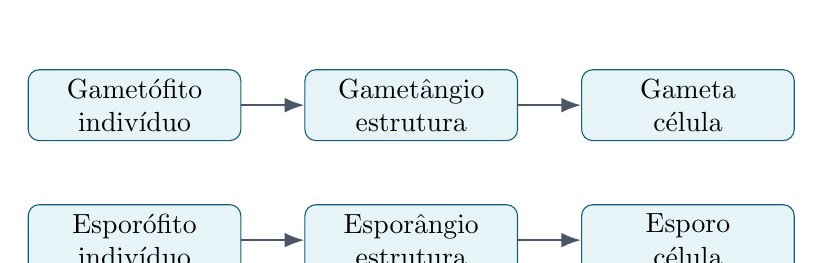
\begin{tikzpicture}[node distance=8mm and 8mm,
bloco/.style={draw=azul,rounded corners,fill=azulclaro,align=center,
minimum width=2.7cm,minimum height=0.9cm},
arr/.style={-{Latex[length=2.5mm]},thick,draw=cinza}]
\node[bloco] (gf) {Gametófito\\indivíduo};
\node[bloco,right=of gf] (ga) {Gametângio\\estrutura};
\node[bloco,right=of ga] (g) {Gameta\\célula};
\draw[arr] (gf)--(ga);\draw[arr] (ga)--(g);
\node[bloco,below=of gf] (ef) {Esporófito\\indivíduo};
\node[bloco,right=of ef] (ea) {Esporângio\\estrutura};
\node[bloco,right=of ea] (e) {Esporo\\célula};
\draw[arr] (ef)--(ea);\draw[arr] (ea)--(e);
\end{tikzpicture}
\end{center}

\begin{essencial}
\textbf{Gameta precisa fundir-se para formar zigoto. Esporo germina sem fusão.}
Esporo não é gameta e não existe esporo masculino ou feminino.
\end{essencial}

\section{Ciclos de vida: conteúdo confirmado para a prova}
A pergunta decisiva é: \textbf{onde ocorre a meiose?} Há três tipos básicos
--- haplôntico, diplôntico e haplodiplôntico ---, mas o último aparece aqui em
duas formas importantes: bifásica e trifásica.

\subsection{Haplôntico: meiose zigótica}
O adulto haploide produz gametas por \textbf{mitose}. A fecundação forma o
zigoto, única fase diploide. O zigoto sofre meiose.

\begin{center}
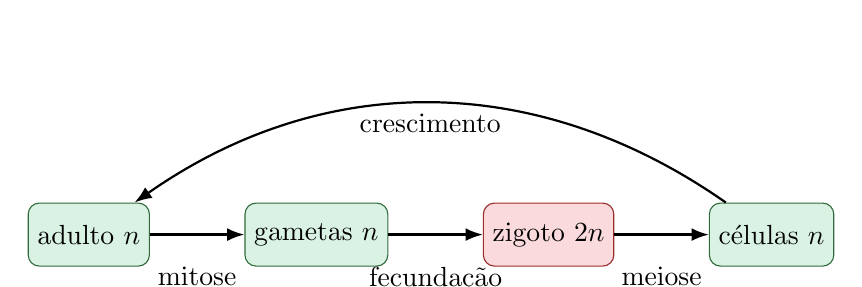
\begin{tikzpicture}[node distance=12mm and 12mm,
h/.style={draw=verde,fill=haploide,rounded corners,minimum height=8mm},
d/.style={draw=vermelho,fill=diploide,rounded corners,minimum height=8mm},
arr/.style={-{Latex[length=2.2mm]},thick}]
\node[h] (a) {adulto \n};\node[h,right=of a] (g) {gametas \n};
\node[d,right=of g] (z) {zigoto \dn};\node[h,right=of z] (c) {células \n};
\draw[arr] (a)--node[below,yshift=-8pt]{mitose}(g);
\draw[arr] (g)--node[below, yshift=-8pt]{fecundação}(z);
\draw[arr] (z)--node[below, yshift=-8pt]{meiose}(c);
\draw[arr] (c) to[bend right=35] node[below]{crescimento} (a);
\end{tikzpicture}
\end{center}

\subsection{Diplôntico: meiose gamética}
O adulto diploide produz gametas por \textbf{meiose}. A fase haploide restringe-se
aos gametas. O zigoto diploide cresce por mitoses.

\begin{center}
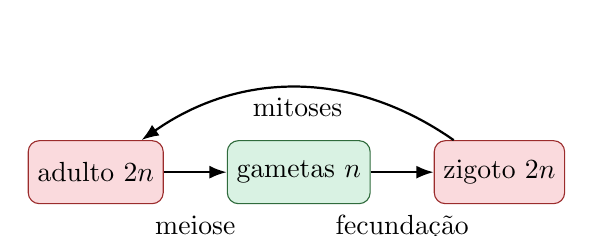
\begin{tikzpicture}[node distance=7mm and 8mm,
h/.style={draw=verde,fill=haploide,rounded corners,minimum height=8mm},
d/.style={draw=vermelho,fill=diploide,rounded corners,minimum height=8mm},
arr/.style={-{Latex[length=2.2mm]},thick}]
\node[d] (a) {adulto \dn};\node[h,right=of a] (g) {gametas \n};
\node[d,right=of g] (z) {zigoto \dn};
\draw[arr] (a)--node[below, yshift=-12pt]{meiose}(g);
\draw[arr] (g)--node[below, yshift=-12pt]{fecundação}(z);
\draw[arr] (z) to[bend right=35] node[below]{mitoses} (a);
\end{tikzpicture}
\end{center}

\subsection{Haplodiplôntico: meiose espórica}
Há gametófito haploide e esporófito diploide. O gametófito produz gametas por
mitose. A fecundação gera o zigoto e depois o esporófito. No esporângio ocorre
meiose, formando esporos haploides.

\begin{center}
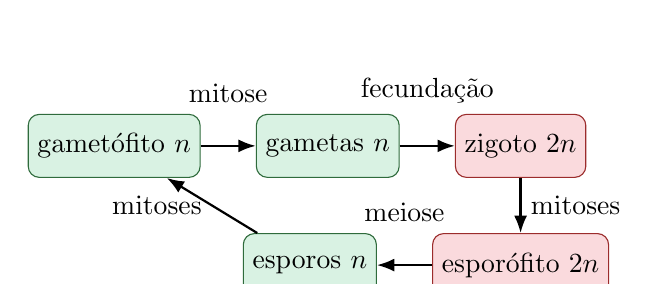
\begin{tikzpicture}[node distance=7mm and 7mm,
h/.style={draw=verde,fill=haploide,rounded corners,minimum height=8mm},
d/.style={draw=vermelho,fill=diploide,rounded corners,minimum height=8mm},
arr/.style={-{Latex[length=2.2mm]},thick}]
\node[h] (gf) {gametófito \n};\node[h,right=of gf] (g) {gametas \n};
\node[d,right=of g] (z) {zigoto \dn};\node[d,below=of z] (ef) {esporófito \dn};
\node[h,left=of ef] (e) {esporos \n};
\draw[arr] (gf)--node[above, yshift=+12pt]{mitose}(g);
\draw[arr] (g)--node[above, yshift=+12pt]{fecundação}(z);
\draw[arr] (z)--node[right]{mitoses}(ef);
\draw[arr] (ef)--node[above, yshift=+12pt]{meiose}(e);
\draw[arr] (e)--node[left]{mitoses}(gf);
\end{tikzpicture}
\end{center}

Gametófito e esporófito podem ser \textbf{isomórficos} (aparência semelhante)
ou \textbf{heteromórficos} (formas diferentes).

\begin{resumo}
\begin{center}
\begin{tabularx}{0.96\textwidth}{>{\bfseries}lCCC}
\toprule
& Haplôntico & Diplôntico & Haplodiplôntico\\
\midrule
Adulto(s) & \n & \dn & \n{} e \dn\\
Fase reduzida & zigoto \dn & gametas \n & nenhuma geração\\
Local da meiose & zigoto & formação dos gametas & esporângio\\
Nome & zigótica & gamética & espórica\\
\bottomrule
\end{tabularx}
\end{center}
\end{resumo}

\begin{essencial}[title={Como reconhecer o ciclo em uma questão}]
\begin{enumerate}
\item Marque a ploidia de cada fase: \n{} ou \dn{}.
\item Localize a fecundação: ela sempre estabelece a fase \dn{}.
\item Localize a meiose: ela sempre restabelece a fase \n{}.
\item Conte as fases multicelulares. No ciclo trifásico das algas vermelhas
há uma fase \n{} e duas fases \dn{}.
\end{enumerate}
\end{essencial}

\begin{landscape}
\thispagestyle{empty}
\begin{center}
{\LARGE\bfseries\color{azul} Esquema geral dos ciclos de vida}\par
\vspace{1mm}
{\small Azul: fase haploide (\n) \qquad Vermelho: fase diploide (\dn)}
\end{center}

\tikzset{
  fasevida/.style={draw,rounded corners=2.5mm,very thick,align=center,
    minimum width=3.15cm,minimum height=1.05cm,fill=white},
  processovida/.style={draw=cinza,rounded corners=1.5mm,thick,align=center,
    fill=cinzaclaro,font=\footnotesize,inner sep=4pt},
  setavida/.style={-{Stealth[length=3mm]},very thick,draw=cinza},
  painelvida/.style={draw=cinza!45,rounded corners=3mm,fill=none,inner sep=6mm}
}

\begin{adjustbox}{max totalsize={\linewidth}{0.78\textheight},center}
\begin{tikzpicture}[font=\small,node distance=9mm and 12mm]
% Haplôntico
\begin{scope}[local bounding box=haplonte]
  \node[fasevida,text=azul] (ha) {\textbf{Adulto haploide}\\\n};
  \node[fasevida,text=azul,right=15mm of ha] (hg) {\textbf{Gametas}\\\n};
  \node[fasevida,text=vermelho,below=17mm of hg] (hz) {\textbf{Zigoto}\\\dn};
  \node[processovida,below=9mm of ha] (hm) {meiose zigótica};
  \draw[setavida] (ha)--node[above, yshift = -20pt, font=\footnotesize]{mitose}(hg);
  \draw[setavida] (hg)--node[right,font=\footnotesize]{fecundação}(hz);
  \draw[setavida] (hz)--(hm); \draw[setavida] (hm)--(ha);
  \node[font=\large\bfseries,text=azul,above=7mm of $(ha)!0.5!(hg)$]{HAPLÔNTICO};
  \node[align=center,font=\footnotesize,below=6mm of $(hm)!0.5!(hz)$]
    {A fase multicelular é haploide.\\Meiose no zigoto.};
\end{scope}
\node[painelvida,fit=(haplonte)]{};

% Diplôntico
\begin{scope}[xshift=14.2cm,local bounding box=diplonte]
  \node[fasevida,text=vermelho] (da) {\textbf{Adulto diploide}\\\dn};
  \node[processovida,right=8mm of da] (dm) {meiose\\gamética};
  \node[fasevida,text=azul,right=8mm of dm] (dg) {\textbf{Gametas}\\\n};
  \node[fasevida,text=vermelho,below=17mm of dg] (dz) {\textbf{Zigoto}\\\dn};
  \draw[setavida] (da)--(dm); \draw[setavida] (dm)--(dg);
  \draw[setavida] (dg)--node[right,font=\footnotesize]{fecundação}(dz);
  \draw[setavida] (dz.south)|-node[pos=.25,below,font=\footnotesize]{mitoses}
    ($(da.south)+(0,-7mm)$)--(da.south);
  \node[font=\large\bfseries,text=vermelho,above=7mm of dm]{DIPLÔNTICO};
  \node[align=center,font=\footnotesize,below=10mm of $(da)!0.5!(dz)$]
    {A fase multicelular é diploide.\\Meiose forma os gametas.};
\end{scope}
\node[painelvida,fit=(diplonte)]{};

% Haplodiplôntico bifásico
\begin{scope}[yshift=-9.55cm,local bounding box=bifasico]
  \node[fasevida,text=azul] (bgf) {\textbf{Gametófito}\\\n};
  \node[fasevida,text=azul,right=13mm of bgf] (bg) {\textbf{Gametas}\\\n};
  \node[fasevida,text=vermelho,right=13mm of bg] (bz) {\textbf{Zigoto}\\\dn};
  \node[fasevida,text=vermelho,below=16mm of bz] (bes) {\textbf{Esporófito}\\\dn};
  \node[fasevida,text=azul,left=13mm of bes] (bsp) {\textbf{Esporos}\\\n};
  \node[processovida,left=13mm of bsp] (bm) {meiose espórica};
  \draw[setavida] (bgf)--node[above,font=\footnotesize]{mitose}(bg);
  \draw[setavida] (bg)--node[above,font=\footnotesize]{fecundação}(bz);
  \draw[setavida] (bz)--node[right,font=\footnotesize]{mitoses}(bes);
  \draw[setavida] (bes)--(bsp); \draw[setavida] (bsp)--(bm);
  \draw[setavida] (bm)--node[left,font=\footnotesize]{germinação}(bgf);
  \node[font=\large\bfseries,text=verde,above=7mm of bg]
    {HAPLODIPLÔNTICO BIFÁSICO};
  \node[align=center,font=\footnotesize,below=6mm of bsp]
    {Gametófito e esporófito multicelulares.\\Podem ser isomórficos ou heteromórficos.};
\end{scope}
\node[painelvida,fit=(bifasico)]{};

% Haplodiplôntico trifásico
\begin{scope}[xshift=14.2cm,yshift=-9.55cm,local bounding box=trifasico]
  \node[fasevida,text=azul] (tgf) {\textbf{Gametófito}\\\n};
  \node[fasevida,text=azul,right=12mm of tgf] (tgam) {\textbf{Gametas}\\\n};
  \node[fasevida,text=vermelho,right=12mm of tgam] (tz) {\textbf{Zigoto}\\\dn};
  \node[fasevida,text=vermelho,below=14mm of tz] (tc) {\textbf{Carposporófito}\\\dn};
  \node[fasevida,text=vermelho,below=14mm of tgam] (tcp) {\textbf{Carpósporos}\\\dn};
  \node[fasevida,text=vermelho,below=14mm of tgf] (tt) {\textbf{Tetrasporófito}\\\dn};
  \node[processovida,below=9mm of tt] (tme) {meiose};
  \node[fasevida,text=azul,right=12mm of tme] (tsp) {\textbf{Tetrásporos}\\\n};
  \draw[setavida] (tgf)--node[above,font=\footnotesize]{mitose}(tgam);
  \draw[setavida] (tgam)--node[above,font=\footnotesize]{fecundação}(tz);
  \draw[setavida] (tz)--(tc);
  \draw[setavida] (tc)--node[right,font=\footnotesize]{mitoses}(tcp);
  \draw[setavida] (tcp)--(tt); \draw[setavida] (tt)--(tme);
  \draw[setavida] (tme)--(tsp);
  \draw[setavida] (tsp.west)--++(-6mm,0)|-
    node[pos=.75,left,font=\footnotesize]{germinação}($(tgf.west)+(-7mm,0)$)--(tgf.west);
  \node[font=\large\bfseries,text=verde,above=7mm of tgam]
    {HAPLODIPLÔNTICO TRIFÁSICO};
  \node[align=center,font=\footnotesize,below=6mm of tsp]
    {Gametófito, carposporófito e tetrasporófito.\\Típico de muitas algas vermelhas.};
\end{scope}
\node[painelvida,fit=(trifasico)]{};
\end{tikzpicture}
\end{adjustbox}
\end{landscape}


\section{Comparação dos três grandes grupos}
Os nomes servem aqui para organizar características, não para cobrar hierarquia
taxonômica.

\begin{longtable}{>{\bfseries}p{0.15\textwidth}p{0.235\textwidth}p{0.235\textwidth}p{0.235\textwidth}}
\toprule
Item & Verdes & Pardas & Vermelhas\\
\midrule
\endfirsthead
\toprule
Item & Verdes & Pardas & Vermelhas\\
\midrule
\endhead
Pigmentos & clorofilas \textit{a} e \textit{b}; carotenoides & clorofilas
\textit{a} e \textit{c}; fucoxantina & clorofila \textit{a};
ficobiliproteínas\\
Reserva & amido dentro do cloroplasto & laminarina e manitol & amido das
florídeas no citoplasma\\
Parede & principalmente celulose; pode haver outros polímeros e CaCO$_3$ &
celulose e componentes algínicos; pode haver CaCO$_3$ & celulose e matriz
mucilaginosa com polissacarídeos sulfatados; pode haver CaCO$_3$\\
Flagelos & presentes em alguma fase de muitas espécies & gametas e/ou esporos
com flagelos heterocontes & ausentes em todas as fases\\
Plastos & duas membranas; endossimbiose primária & quatro membranas;
endossimbiose secundária envolvendo ancestral vermelho & duas membranas;
endossimbiose primária\\
Habitat & grupo com muitas formas dulcícolas; macroalgas marinhas sobretudo
tropicais e subtropicais & quase todas marinhas; muito representativas em águas
frias e temperadas & predominantemente marinhas e bentônicas; ampla distribuição
e ocorrência em maior profundidade\\
Talo & filamentoso, sifonoso, laminar e calcificado & sempre multicelular;
filamentoso a parenquimatoso, incluindo kelps & filamentoso,
pseudoparenquimatoso, laminar e frequentemente calcificado\\
Ciclos & haplôntico, diplôntico ou haplodiplôntico & diplôntico ou
haplodiplôntico & haplodiplôntico bifásico ou trifásico\\
Produto marcante & alimento, fertilizantes e biofiltros & alginato; kombu e
wakame & ágar e carragenanas; nori\\
\bottomrule
\end{longtable}

\begin{essencial}
\textbf{Verde:} amido no cloroplasto. \textbf{Parda:} laminarina e manitol.
\textbf{Vermelha:} amido das florídeas fora do cloroplasto.
\end{essencial}

\section{Algas verdes e pardas: síntese orientada}

\subsection{Algas verdes}
Apresentam clorofilas \textit{a} e \textit{b}, amido no cloroplasto e parede
predominantemente celulósica. Entre as macroalgas marinhas, aparecem talos
filamentosos, cenocíticos, laminares e calcificados.

Talos cenocíticos podem alcançar grande tamanho mesmo sendo uma única célula
multinucleada. Talos laminares, como os de \textit{Ulva}, possuem grande área
para luz e nutrientes e crescem rapidamente em ambientes eutrofizados. Formas
calcificadas contribuem para sedimentos carbonáticos e resistem à herbivoria.

Podem apresentar fragmentação, zoósporos ou aplanósporos e reprodução sexuada
por isogamia, anisogamia ou oogamia. O grupo reúne ciclos haplônticos,
diplônticos e haplodiplônticos; \textit{Ulva} pode apresentar alternância
isomórfica.

Ecologicamente, são produtoras, participam da ciclagem de nutrientes, alimentam
herbívoros, formam micro-habitats e estabilizam substratos. Economicamente, são
usadas como alimento, ração, fertilizante, bioestimulante, biofiltro e fonte de
compostos bioativos.

\subsection{Algas pardas}
São multicelulares, predominantemente marinhas e bentônicas. A fucoxantina,
junto às clorofilas \textit{a} e \textit{c}, explica a coloração parda. As
reservas são laminarina e manitol. Na parede, celulose fornece suporte e
componentes algínicos formam uma matriz hidratada que ajuda contra a dessecação.

A diversidade vai de talos filamentosos microscópicos a kelps parenquimatosos
com dezenas de metros. Pneumatocistos aumentam a flutuabilidade e mantêm lâminas
próximas da luz. Gametas ou esporos móveis possuem flagelos heterocontes,
geralmente um plumoso e outro liso.

Os ciclos são diplônticos ou haplodiplônticos. Nas kelps, a alternância costuma
ser heteromórfica: esporófito grande e gametófito microscópico.

Florestas de kelps criam habitat tridimensional e sustentam cadeias tróficas. O
\textbf{alginato} é usado como espessante, emulsificante e estabilizante em
alimentos, fármacos, tintas e outros produtos. Há alimentos como kombu e wakame
e compostos de interesse biotecnológico.

\section{Algas vermelhas: núcleo principal da prova}

\subsection{Características distintivas}
\begin{itemize}
\item predominância marinha e bentônica; formas epífitas, epizóicas, endófitas e
parasitas;
\item clorofila \textit{a} e ficobiliproteínas em ficobilissomos;
\item pigmentos acessórios que aproveitam luz disponível em maior profundidade;
\item ausência completa de flagelos;
\item amido das florídeas no citoplasma, fora do cloroplasto;
\item parede com celulose e matriz de polissacarídeos sulfatados, fonte de ágar
e carragenanas;
\item conexões celulares (\textit{pit connections}), relacionadas sobretudo à
união mecânica entre células;
\item formas filamentosas, pseudoparenquimatosas, laminares e calcificadas.
\end{itemize}

Formas calcárias podem ser articuladas, com regiões não calcificadas flexíveis,
ou crostosas não articuladas. \textbf{Rodólitos} são nódulos formados
predominantemente por algas vermelhas coralinas e constituem habitats bentônicos
complexos.

\subsection{Reprodução sexuada sem flagelos}
O \textbf{esperma\-tângio} produz o \textbf{espermácio} haploide, gameta masculino
sem flagelo, transportado passivamente. A estrutura feminina é o
\textbf{carpogônio}; sua extensão receptora é a \textbf{tricógine}.
\[
\text{espermácio }(n)+\text{núcleo do carpogônio }(n)
\longrightarrow \text{zigoto }(2n).
\]

\subsection{Ciclo trifásico passo a passo}
O ciclo trifásico possui \textbf{três fases multicelulares}: um gametófito
haploide e dois esporófitos diploides. É exclusivo das Rhodophyta, mas não
ocorre em todas as algas vermelhas.

\begin{enumerate}[label=\textbf{Etapa \arabic*:}]
\item Gametófitos masculino e feminino \n{} produzem gametas \n{} por
\textbf{mitose}.
\item O espermácio alcança a tricógine. A fecundação gera o zigoto \dn.
\item O zigoto fica ligado ao gametófito feminino e origina o
\textbf{carposporófito} \dn.
\item O carposporófito forma por mitose muitos \textbf{carpósporos} \dn. O
conjunto protegido por tecidos do gametófito feminino constitui o
\textbf{cistocarpo}.
\item O carpósporo germina e origina o \textbf{tetrasporófito} \dn,
geralmente livre.
\item Nos \textbf{tetrasporângios} ocorre meiose, formando quatro
\textbf{tetrásporos} \n.
\item Os tetrásporos germinam e originam gametófitos \n.
\end{enumerate}

\begin{center}
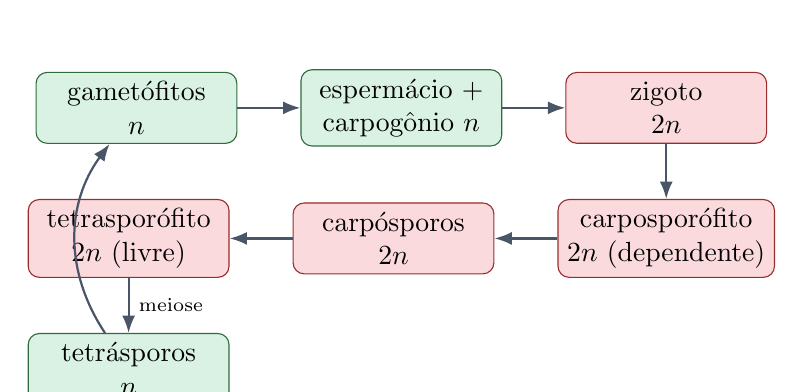
\begin{tikzpicture}[node distance=7mm and 8mm,
h/.style={draw=verde,fill=haploide,rounded corners,align=center,
minimum width=2.55cm,minimum height=9mm},
d/.style={draw=vermelho,fill=diploide,rounded corners,align=center,
minimum width=2.55cm,minimum height=9mm},
arr/.style={-{Latex[length=2.2mm]},thick,draw=cinza},
lab/.style={font=\scriptsize,align=center}]
\node[h, xshift=-20] (gf) {gametófitos\\\n};
\node[h,right=of gf] (gam) {espermácio +\\carpogônio \n};
\node[d,right=of gam] (zig) {zigoto\\\dn};
\node[d,below=of zig] (carp) {carposporófito\\\dn{} (dependente)};
\node[d,left=of carp] (cp) {carpósporos\\\dn};
\node[d,left=of cp] (tet) {tetrasporófito\\\dn{} (livre)};
\node[h,below=of tet] (ts) {tetrásporos\\\n};
\draw[arr] (gf)--(gam);
\draw[arr] (gam)--(zig);
\draw[arr] (zig)--(carp);
\draw[arr] (carp)--(cp);
\draw[arr] (cp)--(tet);
\draw[arr] (tet)--node[right,lab]{meiose}(ts);
\draw[arr] (ts) to[bend left=35] (gf);
\end{tikzpicture}
\end{center}

\begin{essencial}[title={Frase para memorizar o ciclo trifásico}]
\textbf{Gametófito faz gametas; fecundação forma carposporófito; carposporófito
faz carpósporos; carpósporos formam tetrasporófito; tetrasporófito faz meiose e
tetrásporos; tetrásporos formam gametófitos.}
\end{essencial}

\subsection{Vantagem do carposporófito}
A ausência de flagelos torna o encontro dos gametas dependente do transporte
passivo. Depois de uma fecundação bem-sucedida, o carposporófito multiplica
mitoticamente o produto diploide e libera muitos carpósporos. Assim,
\textbf{uma fecundação é amplificada em muitos propágulos diploides}.

\begin{cuidado}[title={Erros clássicos no ciclo das vermelhas}]
\begin{itemize}
\item Carpósporo é \dn, não \n.
\item Tetrásporo é \n, pois resulta de meiose.
\item A meiose ocorre no tetrasporângio, não no carposporófito.
\item O carposporófito \dn{} permanece ligado ao gametófito feminino \n.
\item Cistocarpo reúne o carposporófito e tecidos associados do gametófito
feminino; não é apenas outro nome para carposporófito.
\item Espermácio é o gameta masculino aflagelado; carpogônio é a estrutura
feminina cuja tricógine o recebe.
\end{itemize}
\end{cuidado}

\subsection{Importância das vermelhas}
Como produtoras primárias, fixam carbono, liberam oxigênio e alimentam
consumidores. Formas coralinas ajudam a construir e cimentar recifes; bancos de
rodólitos formam habitat e participam da dinâmica do carbono e dos sedimentos.

Na economia, destacam-se o nori, o \textbf{ágar/agarose} empregado como
gelificante e em meios de cultura, e as \textbf{carragenanas} usadas como
espessantes, estabilizantes e emulsificantes. Há usos em cosméticos, rações,
adubos, corretivos de solo e biofiltros.

\section{Importância ecológica e econômica}

\subsection{Importância ecológica}
\begin{enumerate}
\item \textbf{Produção primária:} convertem energia luminosa em matéria
orgânica, sustentando cadeias alimentares e produzindo oxigênio.
\item \textbf{Engenharia de habitat:} kelps, rodólitos e talos ramificados
criam abrigo e áreas de alimentação e reprodução.
\item \textbf{Ciclagem de nutrientes:} incorporam nutrientes dissolvidos e os
redistribuem pela teia trófica e decomposição.
\item \textbf{Ciclo do carbono:} fixam CO$_2$; formas calcárias participam da
dinâmica de depósitos carbonáticos.
\item \textbf{Estrutura costeira:} formas calcárias consolidam recifes e outros
talos podem estabilizar sedimentos.
\item \textbf{Indicação ambiental:} mudanças de abundância e florações podem
refletir eutrofização e qualidade da água.
\end{enumerate}

\begin{raciocinio}
Não responda apenas que produzem oxigênio e servem de alimento. Acrescente o
mecanismo e a consequência: talos tridimensionais aumentam a complexidade do
habitat, oferecendo abrigo e áreas de alimentação.
\end{raciocinio}

\subsection{Produtos e aplicações}
\begin{center}
\begin{tabularx}{\textwidth}{>{\bfseries}p{0.18\textwidth}p{0.20\textwidth}YY}
\toprule
Produto/uso & Fonte & Função & Exemplos\\
\midrule
Alginato & algas pardas & espessante, estabilizante e emulsificante & sorvetes,
panificação, tintas e fármacos\\
Ágar/agarose & algas vermelhas & gelificante e suporte sólido & alimentos, meios
de cultura e biotecnologia\\
Carragenanas & algas vermelhas & espessante, estabilizante e emulsificante &
alimentos, cosméticos e fármacos\\
Alimento & três grupos & nutrição e ingredientes & nori, kombu e wakame\\
Biofiltro & verdes e vermelhas em cultivo integrado & remoção de nutrientes &
aquicultura multitrófica\\
Fertilizante & vários grupos & minerais e compostos bioativos & agricultura\\
\bottomrule
\end{tabularx}
\end{center}

\section{Quadro-mestre para a véspera}
\begin{longtable}{>{\bfseries}p{0.23\textwidth}p{0.68\textwidth}}
\toprule
Pergunta & Resposta mínima correta\\
\midrule
\endfirsthead
\toprule
Pergunta & Resposta mínima correta\\
\midrule
\endhead
O que é talo? & Corpo vegetativo sem raiz, caule e folhas verdadeiros e sem
sistema vascular típico das plantas terrestres.\\
Por que a forma importa? & Controla luz, nutrientes, arrasto, dessecação e
herbivoria; determina o desempenho ecológico.\\
Gameta ou esporo? & Gameta funde-se; esporo germina sem fusão.\\
Haplôntico & Adulto \n; zigoto é a fase \dn; meiose zigótica.\\
Diplôntico & Adulto \dn; gametas são a fase \n; meiose gamética.\\
Haplodiplôntico & Gametófito \n{} e esporófito \dn; meiose espórica.\\
Verdes & Clorofilas \textit{a}/\textit{b}, amido no cloroplasto, grande
diversidade de talos e ciclos.\\
Pardas & Clorofilas \textit{a}/\textit{c} e fucoxantina, laminarina/manitol,
alginatos, ciclos diplônticos ou haplodiplônticos.\\
Vermelhas & Ficobiliproteínas, ausência de flagelos, amido das florídeas fora do
cloroplasto, ágar/carragenanas, ciclos bifásicos ou trifásicos.\\
Sequência trifásica & Gametófito \n{} $\rightarrow$ carposporófito \dn{}
$\rightarrow$ carpósporos \dn{} $\rightarrow$ tetrasporófito \dn{}
$\xrightarrow{\text{meiose}}$ tetrásporos \n{} $\rightarrow$ gametófito \n.\\
Vantagem do carposporófito & Amplifica uma fecundação, produzindo muitos
carpósporos diploides por mitose.\\
Função ecológica & Produção primária, habitat, cadeias tróficas, ciclagem de
nutrientes e carbono e estruturação ambiental.\\
Produtos-chave & Pardas: alginato. Vermelhas: ágar e carragenanas.\\
\bottomrule
\end{longtable}

\section{Revisão ativa}
Tente responder sem consultar as seções anteriores.

\subsection{Perguntas curtas}
\begin{enumerate}
\item Por que apressório, estipe e lâmina não são raiz, caule e folha?
\item Compare vantagem e desvantagem de alta relação superfície/volume.
\item Por que o talo crostoso é vantajoso sob forte hidrodinamismo?
\item Diferencie fragmentação, esporulação e reprodução gamética.
\item Diferencie gameta de esporo.
\item Para cada um dos quatro esquemas estudados, indique a fase multicelular
e o local da meiose.
\item Em qual ciclo o adulto produz gametas por meiose? Em qual produz por
mitose?
\item O que significa alternância isomórfica?
\item Quais pigmentos e reservas caracterizam verdes, pardas e vermelhas?
\item Qual grupo não apresenta fase flagelada?
\item Por que ficobiliproteínas favorecem ocorrência em maior profundidade?
\item Descreva as três fases multicelulares do ciclo trifásico.
\item Onde ocorre meiose nesse ciclo e qual é o produto?
\item Por que carpósporos são diploides?
\item Qual é a relação entre carposporófito e gametófito feminino?
\item Qual a vantagem adaptativa do carposporófito?
\item Associe alginato, ágar e carragenana à origem e a um uso.
\item Explique duas funções ecológicas com causa e consequência.
\item Por que rodólitos são importantes?
\end{enumerate}

\subsection{Verdadeiro ou falso --- corrija as falsas}
\begin{enumerate}
\item No ciclo haplôntico, os gametas são produzidos por meiose.
\item Todo esporo é haploide.
\item No ciclo diplôntico, os gametas são a única fase haploide.
\item O carposporófito produz carpósporos haploides por meiose.
\item O tetrasporófito é diploide e produz tetrásporos haploides.
\item Algas vermelhas possuem espermácios flagelados.
\item O amido das florídeas é armazenado fora do cloroplasto.
\item Alginato é mais associado às algas pardas.
\item A calcificação só tem importância econômica.
\item Um talo cenocítico pode ser grande sem ser multicelular.
\end{enumerate}

\begin{raciocinio}[title={Questão discursiva-síntese}]
Explique o ciclo trifásico, indicando ploidia, estruturas, produtos, local da
meiose e vantagem do carposporófito. Acrescente duas características gerais e
uma importância ecológica e econômica das algas vermelhas.
\end{raciocinio}

\newpage
\section{Gabarito comentado}

\subsection{Perguntas curtas}
\begin{enumerate}
\item São estruturas análogas: cumprem funções semelhantes, mas não possuem a
origem nem a organização vascular dos órgãos das plantas terrestres.
\item Favorece luz e nutrientes, mas aumenta vulnerabilidade mecânica e à
herbivoria.
\item Perfil baixo e forte aderência diminuem arrasto e remoção pelas ondas.
\item Fragmentação usa partes do talo; esporulação forma esporos; reprodução
gamética envolve fecundação.
\item Gameta funde-se; esporo germina diretamente.
\item Haplôntico: adulto \n{} e meiose zigótica; diplôntico: adulto \dn{} e
meiose gamética; haplodiplôntico bifásico: gametófito \n{} e esporófito \dn{},
com meiose espórica; haplodiplôntico trifásico: gametófito \n{},
carposporófito \dn{} e tetrasporófito \dn{}, com meiose no tetrasporângio.
\item No diplôntico, por meiose. No haplôntico, por mitose.
\item Gametófito e esporófito possuem aparência semelhante.
\item Verdes: clorofilas \textit{a}/\textit{b} e amido no cloroplasto. Pardas:
clorofilas \textit{a}/\textit{c}, fucoxantina, laminarina e manitol.
Vermelhas: clorofila \textit{a}, ficobiliproteínas e amido das florídeas no
citoplasma.
\item Rhodophyta.
\item Ampliam o espectro de absorção e aproveitam luz azul-esverdeada que
penetra mais profundamente.
\item Gametófito \n, carposporófito \dn{} e tetrasporófito \dn.
\item No tetrasporângio; produz tetrásporos \n.
\item São formados mitoticamente pelo carposporófito \dn.
\item O carposporófito desenvolve-se sobre o gametófito feminino.
\item Multiplica o resultado de uma fecundação em muitos carpósporos.
\item Alginato: pardas, espessante ou estabilizante. Ágar e carragenanas:
vermelhas, gelificantes ou estabilizantes em alimentos, meios de cultura,
cosméticos ou fármacos.
\item Exemplos: produção primária sustenta consumidores; talos complexos criam
abrigo; incorporação de nutrientes participa da ciclagem; formas calcárias
estruturam recifes.
\item Formam habitats bentônicos, abrigam espécies e participam da dinâmica do
carbono e dos sedimentos carbonáticos.
\end{enumerate}

\subsection{Verdadeiro ou falso}
\begin{enumerate}
\item \textbf{Falso.} O adulto haploide produz gametas por mitose; a meiose é
zigótica.
\item \textbf{Falso.} Esporos podem ser haploides ou diploides.
\item \textbf{Verdadeiro.}
\item \textbf{Falso.} Produz carpósporos \dn{} por mitose.
\item \textbf{Verdadeiro.}
\item \textbf{Falso.} Espermácios não possuem flagelo.
\item \textbf{Verdadeiro.}
\item \textbf{Verdadeiro.}
\item \textbf{Falso.} Também fornece sustentação, defesa, sedimentos e
estrutura recifal.
\item \textbf{Verdadeiro.}
\end{enumerate}

\section*{Fontes do conteúdo}
\addcontentsline{toc}{section}{Fontes do conteúdo}
Guia elaborado a partir das seis aulas fornecidas: introdução às macroalgas;
processos reprodutivos; diversidade morfológica; Chlorophyta; Phaeophyceae; e
algas vermelhas.

Referências gerais indicadas nas aulas: Raven, Evert e Eichhorn,
\textit{Biologia Vegetal}; Lee, \textit{Phycology}; Reviers,
\textit{Biologia e filogenia das algas}; e Keeling (2013), sobre endossimbioses
plastidiais.

\end{document}
